\documentclass[12pt]{article}
%Dr. Hazrat Ali
%COMSATS University Abbottabad Campus
%http://alihazrat.weebly.com/
%Twitter: https://twitter.com/aliustb
%Tutorial file for 2nd edition of latex workshop
\usepackage{amsmath}
\usepackage{graphicx}
\usepackage{subcaption}
\usepackage{multirow}
\usepackage{enumerate}
\usepackage{cite}
\title{A first document in LaTeX}
\author{Hazrat Ali}
\date{04 May 2019}
%===============================================
\begin{document}

\maketitle
\begin{abstract}
Today is 04 May 2019. On this day, we organized a training workshop on LaTeX document compilation. We now love LaTeX.
\end{abstract}
%
\section{Introduction}
We are attending this workshop at COMSATS University Abbottabad Campus.
\subsection{Organizers}
We can also insert subsection. For example, as I have inserted a subsection here.
The ECE department organized the event with support from director, citc, lab personnels and graduate students.
\subsection{Resource persons}
Dr. Hazrat Ali
\subsection{About COMSATS}
%I would like to itemize the names. So, we can use itemize or enumerate. 
COMSATS University has seven campuses.
\begin{enumerate}
	\item Islamabad Campus
	\item Abbottabad Campus
	\item Attock Campus
	\item Wah Cantt Campus
	\item Lahore Campus
	\item Vehari Campus
	\item Sahiwal Campus
\end{enumerate}

\section{How to write equations?}
To determine the distance between any two points $(x_1, y_1)$ and $(x_2, y_2)$, we use 

%We can use the distance formula
\begin{equation}
\label{eqn: distance}
	d = \sqrt{(x_2 - x_1)^2 + (y_2 - y_1)^2}
\end{equation}
We can also use align. For example;
\begin{align}
	d = \sqrt{(x_2 - x_1)^2 + (y_2 - y_1)^2}
\end{align}
Example on equation having summation sign with limits.
\begin{equation}
f \left( \sum_{i=1}^n X_i \right)
=
f \Biggl( \sum_{j=1}^n Y_j \Biggr)
\end{equation}
\begin{equation}
\int_0^M f(x) dx = \int_0^N
\left(\frac{x}{2}\right) dx
\end{equation}
%%%%%%%%%%%%%%%%%%%%%%%%%%%%%%%%
\subsection{Another long equation}
This equation is picked from GAN paper by Talha Iqbal \& Hazrat Ali.
\begin{equation}
\begin{split}
\stackrel{min}{\theta}\ \stackrel{max}{\gamma} \;L\;(G_{\theta}, D_{\gamma}) \;= \;E_{x,y \Rightarrow p(x,y)} \;[log D_{\gamma}(x,y)] \;\\+ \:E_{y\Rightarrow p(y),z \Rightarrow p(z)} \;[log(1 - D_{\gamma}\:(G_{\theta}(y,z),y))] \;+\\ \;\lambda L_{DEV}(G_{\theta})
\end{split}
\end{equation}

\section{Figures}
Now, we discuss the insertion of figures into our document.
\begin{figure}[ht!]
\centering
\fbox{
\includegraphics[width=0.5\textwidth]{pakflag}} %we can use width=0.8\textwidth
\caption{Flag of Pakistan}
\label{fig:pakflag}
\end{figure}

\begin{figure}[ht!]
\centering
\fbox{
\includegraphics[width=0.5\textwidth]{comsatslogo}} %we can use width=0.8\textwidth
\caption{COMSATS logo (old)}
\label{fig:comsatslogo}
\end{figure}
%

%================================================
\subsection{Side by Side Figures}
We can insert sub-figures within a single figure. For example, we can place two figures side by side, each sub-figure will have a separate sub-caption.
\begin{figure}[!htp]
\centering
	\begin{subfigure}[b]{0.4\textwidth}
	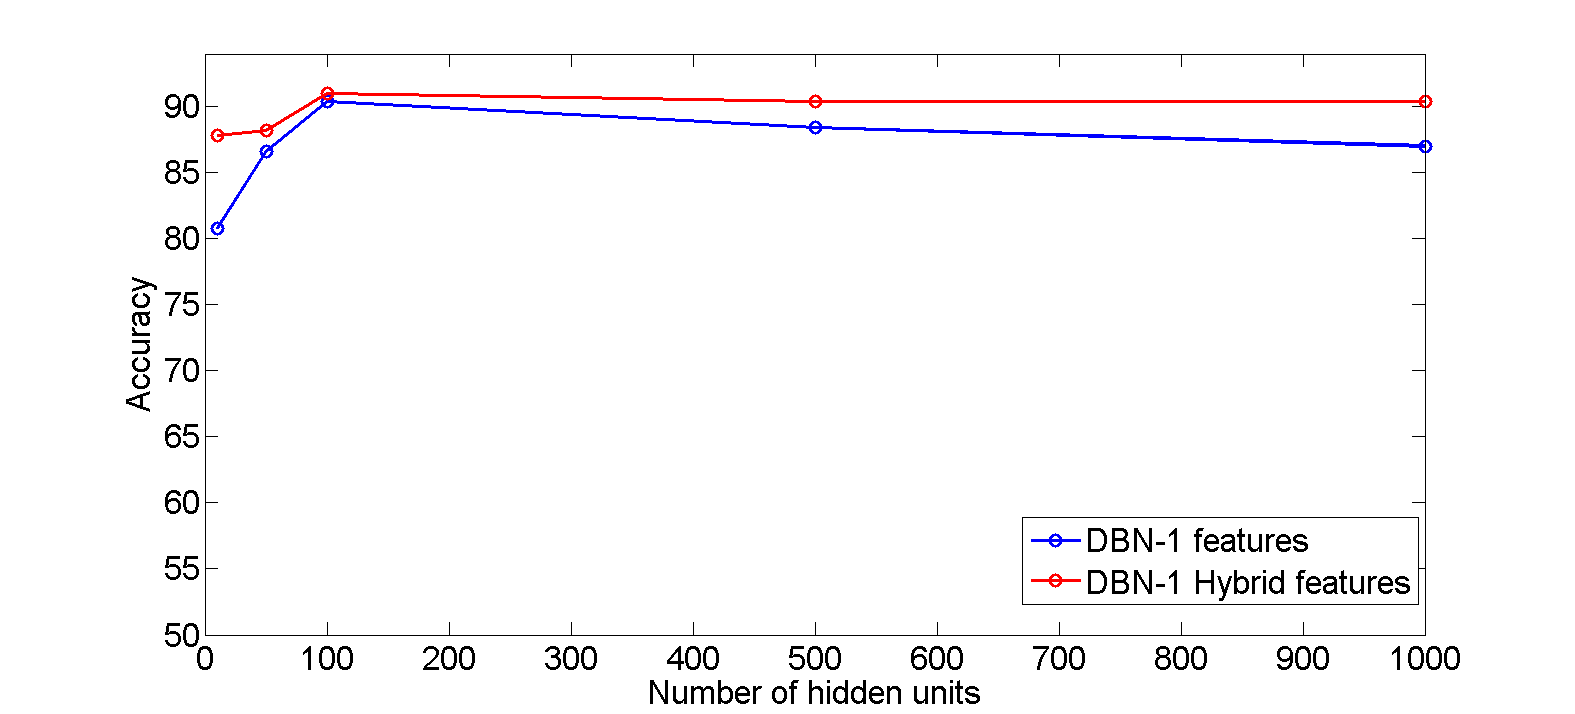
\includegraphics[width=\textwidth]{dbn1_hidden.png}
	\caption{Classification performance DBN1}
	\label{fig:dbn1_hidden} 
	\end{subfigure}
	\qquad \qquad
	\begin{subfigure}[b]{0.4\textwidth}
	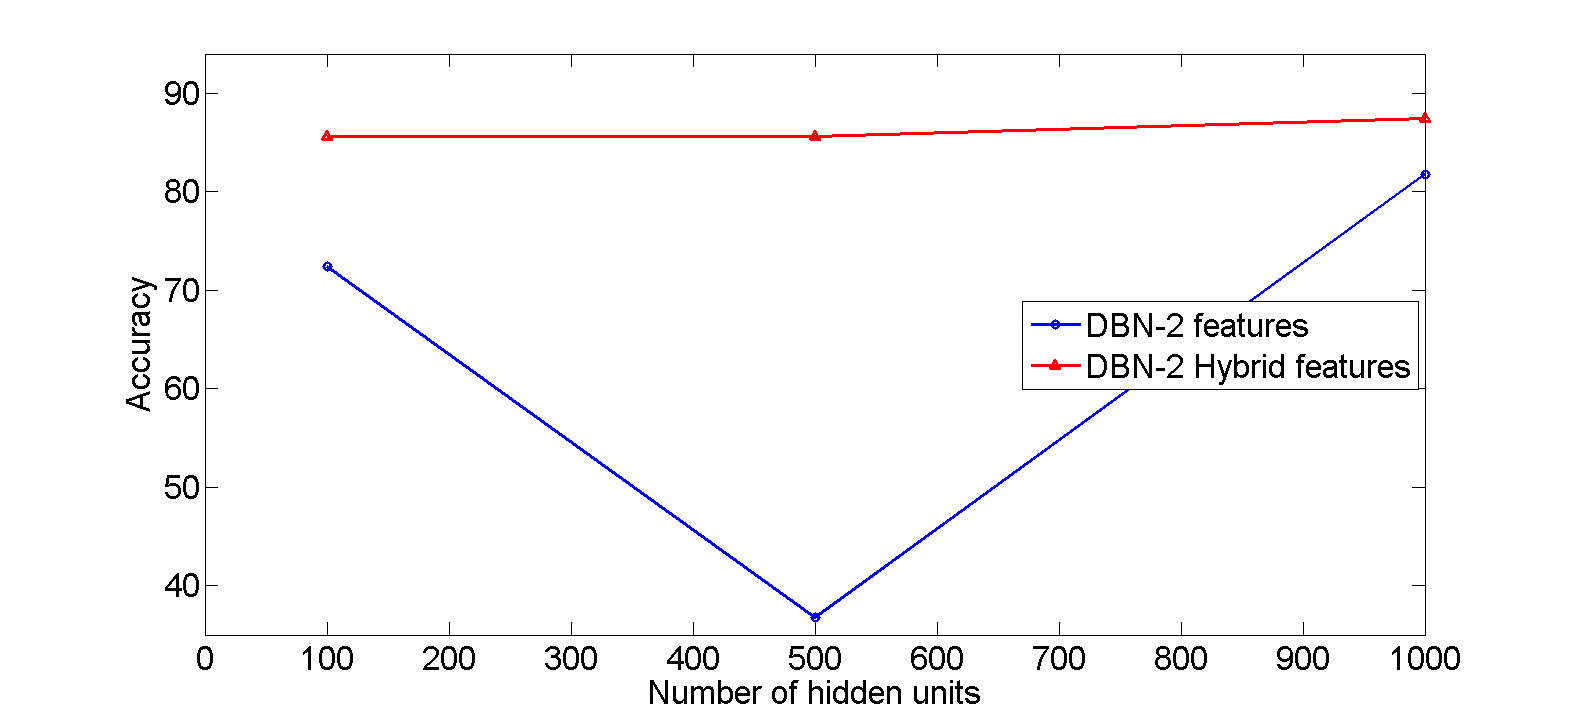
\includegraphics[width=\textwidth]{dbn2_hidden.png}
	\caption{Classification performance DBN2}
	\label{fig:dbn2_hidden} 
	\end{subfigure} 
\caption{Example of two sub-figures}
\end{figure}
%================================
\section{Tables}
We can generate tables by using the tabular environment. A very first example on table.
\begin{table}[h!]
\centering
\caption{Example of a simple table}
\begin{tabular}{|l|l|}
\hline
Student & Marks \\ \hline
Ali & 80 \\
Kamal & 82 \\
Waseem & 73 \\ \hline
\end{tabular}
\end{table}
%%%%%%%%%%%%%%%%%%%
\subsection{Text wrapping in Tables}
\begin{table}[h!]
\centering
\caption{Example of text wrapping in table}
\begin{tabular}{|l|l|p{6cm}|}
\hline
Student & Marks & Comments\\ \hline
Ali & 80 & The student has been regular in class. He improved GPA from 3.3 to 3.5. He is polite. \\ \hline
Kamal & 82 & Kamal is CR for the class. He has good communication skills. He asks questions politely. \\ \hline
Waseem & 73 & Waseem has an impressive hand-writing. His favorite topic is programming.\\ \hline
\end{tabular}
\end{table}
%%%%%%%%%%%%%%%%%%%%%%%%%%%%
%%%%%%%%%%%%%%%%%%%%%%%%%%%%
\begin{table}[h!]
\centering
\caption{Multirows in table}
\begin{tabular}{|l|l|l|}
\hline
Student 							& Subject 		& Marks 	\\ \hline
\multirow{2}{*}{Ali} 	& Mathematics & 80 			\\ 
											& Programming & 85 			\\ \hline
\multirow{2}{*}{Kamal}&Mathematics 	& 73			\\ 
											&Programming 	& 74			 \\  \hline
\multirow{2}{*}{Waseem} &Mathematics & 68				\\ 
											&Programming & 88					\\ \hline
\end{tabular}
\end{table}

\section{Citation}
Now, it is time to discuss citations in latex.  We will generate a new file with .bib extension. Previously, we had a paper in IEEE Access as given in \cite{star2}. 
We are citing our paper published in Springer journal \cite{star1}.
\bibliographystyle{unsrt}
\bibliography{references}
\end{document}
